\documentclass[twocolumn]{article}
\usepackage{graphicx}
\usepackage{tikz}
\usetikzlibrary{positioning,fit}
\usepackage{enumerate}
\usepackage[breaklinks=true]{hyperref}

\begin{document}

\begin{titlepage}

\title{Streaming Query Driven Architecture for \\general Wireless Sensor Networks}
\author{Prakhar Banga \qquad Vineet Hingorani\\\emph{Supervisor:} Prof. Sumit Ganguly}

\maketitle
\date{}

\vfill
\begin{center}

\includegraphics[width=0.40\textwidth]{./IIT_Kanpur_Logo.jpg}
\vfill
\LARGE{Dept. of Computer Science and Engineering, \\IIT Kanpur}

\end{center}
\end{titlepage}



\begin{abstract}
We propose the designing of a general framework for Wireless Sensor Network applications. The framework should be able to reprogram the sensor nodes with reliability, security and keeping in mind that the nodes are constraint over their resources. There have been many approaches towards reprogramming the sensor networks but most of them are not general enough to be able to deploy in a field. The OS used in these works is TinyOS which itself a big constraint to the generality of the work. For now, we plan to study the past works and the developments in the technology to handle a real-time practical system. By being practical, we mean that all of the previous works proposed have been there for theoretical research but have not been commercialized due to their short comings. In practical, the maintenance is done manually and this is where we plan to have an automatic system.
\end{abstract}

\section{Introduction}
Wireless Sensor Networks have a wide range of applications in both the static(from area monitoring to agriculture-based) and dynamic(from military based applications to animal tracking) scenarios. The primary difference between a WSN and a normal wired network is the resource constraints and wireless networking in WSNs. The constraints here are in terms of Power consumption, Computational resources, Memory usage, etc. The sensor nodes in network are very short on their power resource and henceforth their lifetime decreases if they are always ``at work''(sending or receiving data/computing).\\
Most of the information in sensor nets is not needed until something ill has happened, in the sense that most WSNs are event-driven. For example, in a plant health monitoring system, the data sensed by the sensor node(which is normal most of the time) is not needed till the level of plant health has gone below a threshold level(say the nutrient level or temperature etc.) which is a rare event. This problem can be handled by providing the nodes with some computation power and the nodes send their data only when required(say an anomaly has occurred).
Presently, such WSNs have been deployed at huge levels but all of them are domain specific. Development of a WSN framework is usually application dependent where if the program running on a particular node has to changed, it has to be changed manually. On the fly reprogramming has been addressed in many frameworks but as we will show in all of them the assumptions made are not general enough and the \emph{constraint resources} suffer a lot.\\
In Section 2 we will describe the Problem Statement we are going to tackle. Further we elaborate the various issues and problems to be tackled in designing such a framework from different perspectives(OS Level, Networking, etc.). We give some examples of real world applications where these sensor nets are used extensively. We study the previous work in the reprogramming of sensor networks and classify those in terms of the basic issues faced by WSNs.

For a real simulation, we need to have a prototype network of WSNs to test the design of our framework. For that we take Smart Building design as a proof of concept for our work.

\section{Problem statement}
We would like to design a general framework which facilitates and automates manual work required for the deployment and maintenance of WSNs. We want to have a framework such that it is general enough to be used for a lot of applications of WSNs. It should also be programmable so that the job the WSN performs can be changed anytime. Moreover, it should be remotely programmable, so that it can be programmed from a central location. It would also be nice to have the programming paradigm as easy and simple as possible for the programmer.
Currently most of these problems are handled manually and in an ad-hoc manner. A construction of such a general framework would be analogous to the systematization of databases which happened in the 1960s and 70s, when general-purpose database systems emerged.\\
Our final aim is to extend this system to even handle the mobility issues arising from the dynamic WSNs. The basic problem in mobile nodes is the addressing and networking things get complicated. We will have a design keeping in mind the issues faced by mobile networks.

\section{Applications}
WSNs have a wide range of applications. We classify them in two broad areas:
\begin{itemize}
\item Static WSNs: All nodes have a fixed location. e.g.,\
\begin{itemize}
\item Environment monitoring: Environment monitoring usually involves measuring critical aspects of the environment, such as the temperature, humidity, air pressure, radiant light etc. It has a wide impact on the understanding of the environment and habitat dynamics. Our framework would be very useful in deployiong such a system quickly and maintaining it for longer lifetime.
\item Smart buildings: A `smart building' is a building which can automate tasks which humans perform. Human presence sensors and motion sensors can be used for the common job of automatically switching the lights and the air conditioner on and off depending on human presence. Less common tasks like detecting excreta can be used in buildings having animals. We will focus on deploying and maintaining such a system as a proof of concept for our framework.
\item Mechanical monitoring: Mechanical monitoring is the monitoring of physical structures, like machines and bridges. Vibrational patterns of these structures can indicate wear-and-tear and can be used to detect upcoming failure. A lot of resources are wasted today for checking the wear-tear of such machines manually. A WSN, specially reprogrammable, would prove much useful here.
\end{itemize}
\item Dynamic WSNs: Nodes don't have a fixed location. e.g.,\
\begin{itemize}
\item Military monitoring: Dynamic WSNs have wide applications in the military. One application includes monitoring soldier locations which can be critical in times of war or when the soldiers are in certain high-risk areas. Another application is vehicle surveillance, in which military vehicles are fitted with surveillance equipment and they move around collecting data.
\item Animal monitoring: Scientists in their quest to understand the habitat dynamics of certain animals, use trackers to collect data about their whereabouts throughout the year. Such monitoring is done very frequently for bird and fish species and yields a lot of interesting results about their year-round migration.
\item Vehicle tracking: GPS can be used to track vehicles and maintain the locations of a number of vehicles. This can be used by transport companies, in healthcare by tracking ambulances etc.
Of course, the possibilities for WSN applications are endless and any application can be augmented to do other tasks as well.
\end{itemize}
\end{itemize}

The need of programming is everywhere. In military applications, if a soldier is shot, then a program can be changed for the sensor nodes monitoring his health to send the data at the base station regularly and more often as compared to other soldiers. Same in the case of animal tracking system. In `Smart Buildings', reprogramming can help changing the programs or tuning the thresholds in programs running at the nodes in different locations. There is an emense scope and need for reprogramming of these WSN frameworks.

\section{Proposed architecture}
We propose a hierarchical control system(\href{http://en.wikipedia.org/wiki/Hierarchical_control_system}{\nolinkurl{http://en.wikipedia.org/wiki/Hierarchical\_control\_system}})
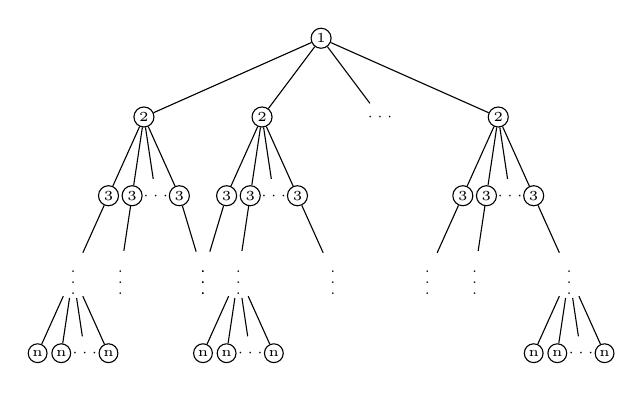
\begin{tikzpicture}[level 1/.style={sibling distance=15mm, level distance=10mm},level 2/.style={sibling distance=3mm},level 3/.style={sibling distance=3mm},level 4/.style={sibling distance=3mm},level 5/.style={sibling distance=3mm},
every node/.style={font=\tiny, circle, inner sep=0.9pt, draw}]
\node[circle,draw] (a) {1}
child{ node [circle,draw] (b) {2}
   child{ node [circle,draw] (c) {3} 
      child{ node [draw=none] (c2) {$\vdots$}
         child{ node [circle,draw] (c21) {n} }
         child{ node [circle,draw] (c22) {n} }
         child{ node [draw=none] (c23) {$\cdots$} }
         child{ node [circle,draw] (c24) {n} }
      }
      child{ node [draw=none] (c1) {} edge from parent[draw=none]}
      child{ node [draw=none] (c3) {} edge from parent[draw=none]}
      child{ node [draw=none] (c4) {} edge from parent[draw=none]}
   }
   child{ node [circle,draw] (d) {3} 
      child{ node [draw=none] {} edge from parent[draw=none]}
      child{ node [draw=none] {$\vdots$} }
      child{ node [draw=none] {} edge from parent[draw=none]}
      child{ node [draw=none] {} edge from parent[draw=none]}
   }
   child{ node [draw=none] (e) {$\cdots$} }
   child{ node [circle,draw] (f) {3} 
      child{ node [draw=none] {} edge from parent[draw=none]}
      child{ node [draw=none] {} edge from parent[draw=none]}
      child{ node [draw=none] {} edge from parent[draw=none]}
      child{ node [draw=none] {$\vdots$} }
      child{ node [draw=none] {} edge from parent[draw=none]}
   }
}
child{ node [circle,draw] (g) {2} 
   child{ node [circle,draw] (h) {3} 
      child{ node [draw=none] {} edge from parent[draw=none]}
      child{ node [draw=none] {$\vdots$} }
      child{ node [draw=none] {} edge from parent[draw=none]}
      child{ node [draw=none] {} edge from parent[draw=none]}
      child{ node [draw=none] {} edge from parent[draw=none]}
   }
   child{ node [circle,draw] (i) {3} 
      child{ node [draw=none] (i1) {} edge from parent[draw=none]}
      child{ node [draw=none] (i2) {$\vdots$}
         child{ node [circle,draw] (i21) {n} }
         child{ node [circle,draw] (i22) {n} }
         child{ node [draw=none] (i23) {$\cdots$} }
         child{ node [circle,draw] (i24) {n} }
      }
      child{ node [draw=none] (i3) {} edge from parent[draw=none]}
      child{ node [draw=none] (i4) {} edge from parent[draw=none]}
   }
   child{ node [draw=none] (j) {$\cdots$} }
   child{ node [circle,draw] (k) {3} 
      child{ node [draw=none] {} edge from parent[draw=none]}
      child{ node [draw=none] {} edge from parent[draw=none]}
      child{ node [draw=none] {} edge from parent[draw=none]}
      child{ node [draw=none] {$\vdots$} }
   }
}
child{ node [draw=none] (l) {$\cdots$} }
child{ node [circle,draw] (m) {2} 
   child{ node [circle,draw](n){3} 
      child{ node [draw=none] {$\vdots$} }
      child{ node [draw=none] {} edge from parent[draw=none]}
      child{ node [draw=none] {} edge from parent[draw=none]}
      child{ node [draw=none] {} edge from parent[draw=none]}
   }
   child{ node [circle,draw](o){3} 
      child{ node [draw=none] {} edge from parent[draw=none]}
      child{ node [draw=none] {$\vdots$} }
      child{ node [draw=none] {} edge from parent[draw=none]}
      child{ node [draw=none] {} edge from parent[draw=none]}
   }
   child{ node [draw=none] (p){$\cdots$} }
   child{ node [circle,draw](q){3} 
      child{ node [draw=none] (q1) {} edge from parent[draw=none]}
      child{ node [draw=none] (q2) {} edge from parent[draw=none]}
      child{ node [draw=none] (q3) {} edge from parent[draw=none]}
      child{ node [draw=none] (q4) {$\vdots$}
         child{ node [circle,draw] (q41) {n} }
         child{ node [circle,draw] (q42) {n} }
         child{ node [draw=none] (q43) {$\cdots$} }
         child{ node [circle,draw] (q44) {n} }
      }
   }
}
;
\end{tikzpicture}

We handle the general case with n layers of nodes, where each node(except the lowest layer):
\begin{itemize}
\item Assigns `tasks' to its children
\item Gathers data from its children
\item Processes the gathered data and sends data back to its parent
\end{itemize}
A node in the lowest layer(i.e.,\ the sensors) sends to the parent either raw sensor data or data processed with the limited processing abilities they have.\\

The `tasks' of these nodes are programs in an SQL-like language aimed at filtering data.\\

Every node has a set of properties, in the form of attribute-value pairs, such as:\\

\begin{tabular}{|l|l|}
\hline
Attribute & Value \\
\hline
A1 & V1 \\
A2 & V2 \\
A3 & V3 \\
\vdots & \vdots \\
Ak & Vk \\
\hline
\end{tabular} \\

These properties can be used for the distribution and diffusion of tasks in the network. For instance, a geographic location property might be used to perform a particular task in a particular area.\\


\section{Programming Paradigm}

In most of the cases the sensor networks are deployed and then any change in the working of sensors need reprogramming in them. There is a need of ‘on-the-fly’ programming of sensor nodes in the sensor networks. Manual reprogramming of a network with thousands of nodes is infeasible. A lot of work has been done in the field of programming of these sensors implementing various wireless routing algorithms that would be useful in such a resource constraint scenario.

There are loads of issues in designing a Programming framework for WSNs. Some of them are:
\begin{enumerate}[a)]
\item \emph{Program Length}: The packets needed to send a large program code would be high and the network congestion increases if large number of packets are send. Also, the power constraints make such communication difficult for the multi-hop sensors. The compute power and memory is also another constraint which will come into place if the Program Code is very big.

\item \emph{Binary Program}: Sending binary program also makes the above issues worse. As said before, the computer power of sensor nodes is very less. Having a compiler at each of the nodes individually is not feasible in a large sensor network and therefore we need to send the large binary code.

\item \emph{Version Control}: The dynamic reprogramming have this issue of different versions for programs at various nodes. This version control can be done at the administrator or at the nodes itself.The design of the framework should be such that the whole network should be scalable and reliable keeping in mind the constraints.

\item \emph{Programming Interface}: The interface for the administrators is also an important issue. It should be easier for a non-programmer to send queries for particular nodes in the network.

\item \emph{Initiation}: There are basically two schemes proposed in the literature of programming these sensors\cite{Wang06reprogrammingwireless}:-
\begin{itemize}
\item \underline{Code Dissemination}- Initiated by the network administrator where code is send to the individual sensors or group of sensors. This could be for various purposes like fixing bugs, changing network structure, changing programs, etc.

\item \underline{Code Acquisition}- This is initiated by sensor nodes themselves as per need or per changing surrounding.
\end{itemize}

The choice depends on what gives you the best performance in overall ways.
\end{enumerate}

\section{Networking}

Wireless Routing has been a great subject of study for the past many years. Issues like reliability, security, quick transmission, etc. are the need for the wireless communication protocols. In the case of WSNs, the requirements for these protocols increase more than mere Wireless networking. Some of the issues faced in routing the packets and networking in WSNs are:
\begin{itemize}
\item \emph{Hops}: To make a general framework the network should be able to handle both the single-hop and multihop transmissions. For remote sensor networks applications, multi hop reprogramming is a need. There are power constraints in nodes that are used frequently to transmit the programs from administrator to far flung nodes in multi hop nets.

\item \emph{Scheduling}: Scheduling issues is also a great concern for reliable and quick transmission. To handle the Hidden Terminal problem we can’t use the conventional solution due to the resource constraints. Avoiding as many collisions as possible is basically the need.

\item \emph{Pipelining}: The framework should be able to pipeline the packets as much as possible. As the packet payload size is very less for, the time taken to send the program to a node 3 hops away from administrator without pipelining would take factors of time more than what it takes with pipeline.

\item \emph{Addressing}: To direct the code to the selected group of nodes, there should be some mechanism for that. Scope Selection\cite{Wang06reprogrammingwireless}\cite{Jeong04incrementalnetwork} is one of the scheme that is done before transmitting the actual program to direct it towards the nodes. Addressing the nodes could also be done. This is an important issue of how to address the nodes and the intricacies behind it.
\end{itemize}

\section{OS Requirements}

As mentioned above, we want our system to be general enough but at the same time it should be very basic. From the perspective of an OS design, we don't need complex Operating System running at the sensor nodes. TinyOS developed by Berkeley and Intel is targeted towards the development of WSNs. It supports a lot of things which really are not needed in most of the Sensor Network applications i.e. the TinyOS is not really tiny. Some of the basic operations that the OS should sopport are given:
\begin{itemize}
\item \emph{Threads}: The OS at the nodes should be able to support threading to listen from many nodes and to send to other nodes. This would be the basic need that an OS for such a framework should support.

\item \emph{Modular}: The OS should be built in a modular fashion to have a support for further extensions. Anything needed for improvement can be added/modified afterwards easily.

\item \emph{File System}: There is no need of file system in the OS. It should be able to run a program on the input data and give the output(nothing more fancy than this).

\item \emph{OSI Model Support}: Reliability is a concern in WSNs. The Transport layer should be as relaible as possible. Scheduling in the MAC layer should be modular so that it could be changed as per needs. TinyOS presently uses simple CSMA, there could be other possibilities also.
\end{itemize}

These are few of the basics from where we can have an insight for a whole operating system. Other than these there are a lot of issues that need to be handled at OS level and this itself could be a great research problem.

\section{Related Work}

A lot of work has been done in network programming mechanisms. These basically address the the major problems:
\begin{itemize}
\item How to program the system?
\item How to send sensor data/programs?
\end{itemize}
We will briefly address some of the past work done in this area.

Motes developed in Berkeley are used extensively for network programming. XNP\cite{mote} is an implementation for TinyOS that broadcasts the whole program to the network and is a single-hop network. The sensor nodes accept the code depending on their needs individually. MOAP\cite{Stathopoulos03aremote} is a multi hop improvement over the XNP. The code dissemination algorithm used in MOAP sends the packets to a few number of nodes rather than flooding the whole network. Deluge\cite{Hui04thedynamic}, MNP\cite{Kulkarni05mnp:multihop} and Aqueduct\cite{citeulike:1990821} does pipelining for sending the packets and improves upon the MOAP. While Deluge and MNP are for the whole network, Aqueduct is for selected number of nodes. Reijer's approach\cite{Reijers03efficientcode} doesn't support pipelining but is a platform dependent scheme using Mate's Virtual Machine Code. Instead of sending the Native code, it sends a VM code that is application specific. This improves upon the number of packets sent but has a disadvantage of computation of the binary mapping at the sensor nodes. It works in a single hop network and floods the network. Trickle\cite{Levis04trickle:a} is an improvement over Reijer's that works on multi-hop networks and doesn't broadcast i.e. flood the network. Incremental\cite{Jeong04incrementalnetwork} approach given by Culler et al. is an approach that updates the programs at the sensor nodes in an incremental manner in such a way that the difference between new program image and old version is computed and writes in the memory are done. This uses a modified version of Rsync algorithm that would work on constraint sensors. TinyCubus\cite{Marrón05managementand} is a scheme that instead of sending the whole program sends the modular updates in the program to the sensor nodes. This improves a lot over the past implementations in terms of power consumption and network communication. The only issue here is that generally programs are not much modular and it is difficult to change the programs in such a way.
\\
The frameworks given described till assume that there is no hierarchy in the network. Firecracker\cite{Levis04thefirecracker} works for a hierarchichal network and is a multi-hop framework. All of these frameworks have been designed for Berkeley Motes and work on TinyOS environment with CSMA as MAC Layer protocol. Sprinkler\cite{Naik05sprinkler:a} is a framework using TDMA as MAC protocol for multi-hop networks and is not designed for the Motes in particular.
\\
The designed frameworks can be put in different categories as described above in the various sections.

\newpage

\bibliographystyle{alpha}
\bibliography{refs}

\end{document}
